\chapter{Controlling vehicle tools}

So far a control system for vehicles is implemented with a GUI. This chapter takes a look on how to proceed with embedding the control system of the associated tools from a vehicle. Since only one model contains an end-effector, the generalised system will be based on the serial manipulator model.

\section{Serial Manipulator}

A virtual model of a robot arm in GeoMod have already been created from earlier student works. This model will be further used in this project as a base to develop a general control system for tools and vehicles. The model of the serial manipulator in GeoMod can be seen in \Cref{fig:SerialManipulator}. The serial manipulator was created from a series of models, created as parts, which is connected with characteristics as linked joints.

\begin{figure}[ht]
    \centering
    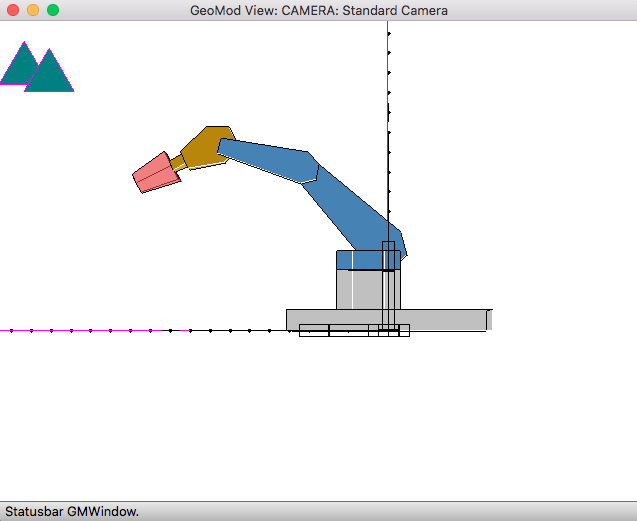
\includegraphics[height=8cm]{images/GeometricModel.png}
    \caption[Geometric model of a serial manipulator]{Geometric model of a serial manipulator}
    \label{fig:SerialManipulator}
\end{figure}


\section{Kinematics}
It was mentioned that from the work of Martin Lygre Fuglevik, the control system for desired position and orientation of objects along a network of paths was partially implemented. Most of the implementation worked as it should, but some occurrence regarding rotation in motion to a particular path did not work as prompted. Some small alteration had to be done in the model in order to continue the implementation of the control system. 

\begin{figure}[ht]
    \centering
    \includegraphics[height=8cm]{images/Diagram_Serial_Manipulator.png}
    \caption[Kinematic connection of  each part of the serial manipulator model]{Kinematic connection of  each part of the serial manipulator model}
    \label{fig:KinematicsSerialManipulator}
\end{figure}


The \Cref{fig:KinematicsSerialManipulator} illutrates how the forward and inverse kinematics works on the implemented model. This is done by having variables over the position, rotation and angle on each part of the model. The angle is determined by linking the parts from the base. By applying forward kinematics, the joints angle is independently controlled for each parts beginning from the position of the linked mechanism, the bracket, to end-effector, the gripper. The function \textit{dirKin()} is an already implemented function that calculate joint angels of all the joints, when one of the joints is moved. This makes a lot of unnecessary computation regarding to joints that are not affected of certain movement. This was disregarded as it did not prevent the objective of this project, but should be taken into account in future for optimization. Forward kinematics works well for a desired end position for the end-effector, but is rather impractical to control when following a path.

To work along network of path, a UAV is prompted to work in a specific area. This means the end-effector of a robot arm on the UAV follow a path as it doing its task. 



